%-----------------------------------------------------------------------------%
\chapter{\babTiga}
%-----------------------------------------------------------------------------%

Penelitian ini dibagi menjadi empat tahap: (1) Mendapatkan data microarray dan pengolahan awal; (2) Perancangan algoritma; (3) Melakukan eksperimen untuk mendapatkan \textit{hyperparameter} yang optimal. Kemudian dilanjutkan dengan  testing dan evaluasi. Gambaran umum dari penelitian ini seperti pada \pic~\ref{fig:overview}




%-----------------------------------------------------------------------------%
\section{Gambaran Umum Penelitian}
%-----------------------------------------------------------------------------%

Secara garis besar, penelitian ini dibagi menjadi beberapa tahapan. Yang pertama adalah tahapan persiapan yaitu mendapatkan data \textit{microarray} kemudian mengolahnya menjadi data yang siap untuk dilakukan proses seleksi fitur dan tahapan pelatihan \textit{deep learning}. Yaitu dengan membagi 80\% data untuk training, 15\% data untuk  validasi dan 5\% data untuk testing.\\
Bagian kedua adalah  membangun model DBN dengan teknik \textit{unsupervised learning}. Untuk mendapatkan model terbaik   secara \textit{greedy} pada tiap-tiap layer RBM-nya. Dimana dilakuan tuning \textit{hyperparameter} (jumlah kedalaman layer, jumlah \textit{hidden unit} pada tiap layernya) digunakan untuk mendapatkan struktur \textit{hyperparameter} yang cocok dengan ciri khas dari data \textit{microarray}. Oleh karena itu diperlukan banyak percobaan untuk mendapatkan hasil yang bagus. \\
Bagian ketiga, adalah \textit{supervised learning}, dimana merupakan  evaluasi sementara dari tahap yang kedua. Dibuat layer output berupa \textit{logistic regression}, yang digunakan untuk menguji sementara hasil dari proses \textit{pretraining} untuk mengklasifikasikan pasien kanker dan pasien normal menggunakan dataset validasi dan dataset testing. \\
Bagian keempat merupakan bagian yang terpenting karena  dimana ide thesis ini dibuat. Yaitu melakukan perankingan gen untuk mencari gen yang paling informatif yang didapatkan dari model pada percobaan sebelumnya. Dimana algoritma seleksi fitur untuk multi-step ranking dijalankan agar didapatkan \textit{biomarker}.\\

\begin{figure}
	\centering
	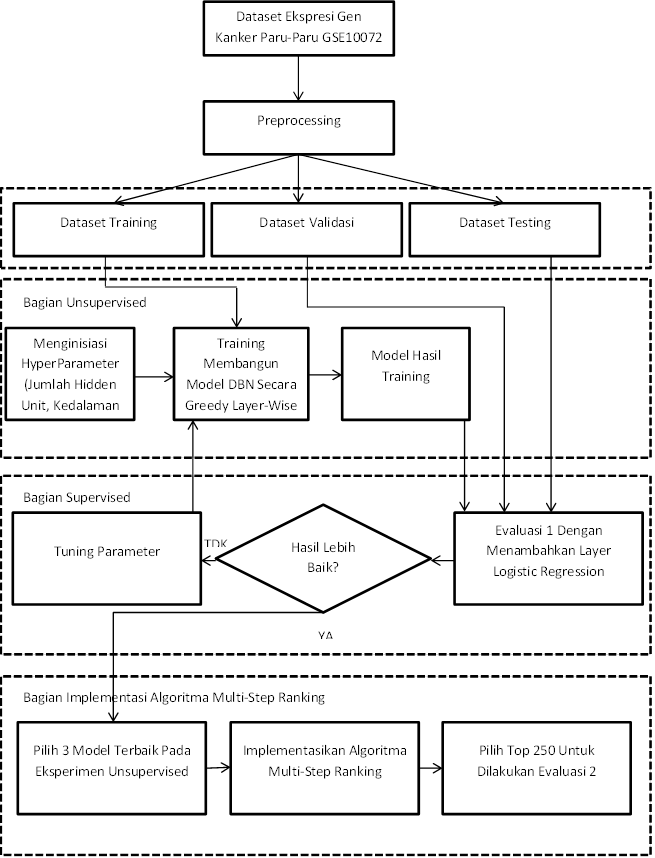
\includegraphics[width=0.9\textwidth]
		{pics/overview.png}
	\caption{Overview Penelitian}
	\label{fig:overview}
\end{figure}

Tahapan terakhir adalah tahap evaluasi akhir, yaitu  akan dilakukan dua kali evaluasi, yang pertama evaluasi  dengan cara membandingkan evaluasi 1 (\textit{logistic regression} sebelum dilakukan seleksi fitur) dengan evaluasi 2 (MLP setelah dilakukan seleksi fitur). Hasil dari kedua proses ini dibandingkan apakah terjadi perbaikan performa klasifikasinya. \\
\begin{figure}
	\centering
	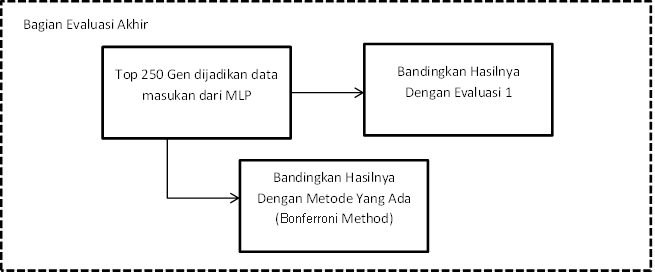
\includegraphics[width=0.9\textwidth]
		{pics/evaluasi2.png}
	\caption{Overview Metode Evaluasi}
	\label{fig:evaluasi2}
\end{figure}
Untuk evaluasi selanjutnya yaitu dilakukan konfirmasi, dimana hasil dari perankingan gen tersebut dibandingkan dengan penelitian tentang biomarker sebelumnya. Apakah gen biomarker yang ditemukan pada penelitian ini memiliki signifikansi dibandingkan dengan teknik sebelumnya.\\
\begin{figure}
	\centering
	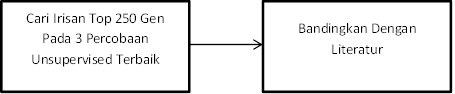
\includegraphics[width=0.8\textwidth]
		{pics/evaluasi3.png}
	\caption{Metode Untuk Mengkonfirmasi Biomarker}
	\label{fig:evaluasi2}
\end{figure}

%-----------------------------------------------------------------------------%
\section{Desain Metode Perangkingan Bobot Secara Multi Step Untuk Mendapatkan Gen Biomarker}
%-----------------------------------------------------------------------------
Pada penelitian ini, akan dibangun sebuah teknik pencarian \textit{Biomarker} dengan metode seleksi fitur gen. Metode ini menerapkan perankingan gen secara \textit{multi step} terhadap model yang didapatkan pada proses \textit{training} yang dilakukan secara \textit{unsupervised}. Arsitektur untuk mendapatkan modelnya adalah digunakan  arsitektur \textit{Deep Belief Network (DBN)} yang merupakan bagian dari metode \textit{deep learning}. Metode perankingan yang digunakan adalah modifikasi dari algoritma seleksi fitur untuk \textit{logistic regression} yang dilakukan oleh \cite{shevade2003simple}. Akan tetapi metode ini memiliki masalah dalam  mengeliminasi fitur jika diterapkan secara langsung pada model DBN, dikarenakan parameter bobot (W) dan bias (b) ditempatkan disetiap fitur dan model ini hanya memiliki satu layer dibandingkan dengan DBN yang memiliki banyak layer. \\
Pada DBN, \textit{hidden unit} yang paling sering aktif adalah \textit{hidden unit} yang lebih penting dibandingkan dengan unit yang jarang aktif, oleh karena itu \textit{hidden unit} ini memiliki parameter bobot yang lebih besar dibandingkan dengan \textit{hidden unit} yang jarang aktif pada saat proses \textit{training} dilakukan. Pemilihan fitur dilakukan dengan meranking unit-unit yang memiliki bobot tertinggi dimulai dari \textit{layer output} mundur secara multi-step menuju \textit{layer input} untuk mendapatkan fitur gen yang paling berpengaruh terhadap model. Kemudian dilakukan eliminasi bobot pada \textit{hidden unit} per layernya secara \textit{multi step}. Selanjutnya akan dipilih sebanyak \textit{top-n} gen dari hasil perankingan ini untuk dievaluasi apakah \textit{Biomarker} yang ditemukan tersebut informatif atau tidak. Seperti digambarkan pada bagan \pic~\ref{fig:multistep1} \\

\begin{figure}
	\centering
	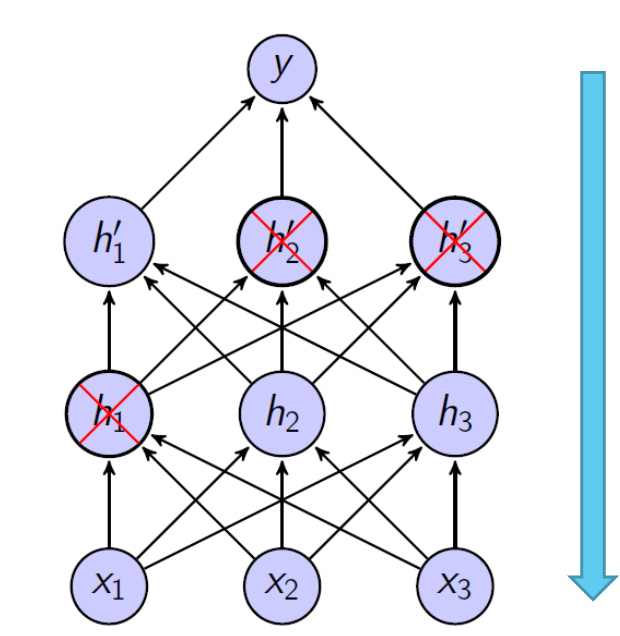
\includegraphics[width=0.3\textwidth]
		{pics/multistep1.png}
	\caption{Hidden unit yang paling sering aktif adalah neuron yang paling penting. Sedangkan yang Kurang Penting Dihapus dengan arah mundur Secara Multi-step \citep{duh2014deep}}
	\label{fig:multistep1}
\end{figure}

\subsection{ Desain Algoritma Multi-Step Ranking }


Input : matrix yang berisi bobot dan bias \\
Output : Matrix yang berisi index gen dan ranking nya \\
\lstset{language=python}          % Set your language (you can change the language for each code-block optionally)

\begin{lstlisting}
# hsl_ranking = multisteprank(model, KonfigurasiLayer):

ekstraktor = Ekstraktor()

model = InputModel

Wlayer3 = model.rbm_layers[3].W
Wlayer2 = model.rbm_layers[2].W
Wlayer1 = model.rbm_layers[1].W
Wlayer0 = model.rbm_layers[0].W

y3 = Wlayer3.get_value(True)
x3 = T.fmatrix()
x3 = y3.copy()

# ranking ujung (Layer 3)
awal3 = mtr.awal(x3)
jml_bobot3 = mtr.jumlah_bobot(x3, awal3)
ranking_jml_bobot3 = mtr.rank_hasil_jumlah(jml_bobot3)
top_n3 = mtr.set_top_n(ranking_jml_bobot3,70)

# ranking layer selanjutnya sampai layer = 0
y2 = Wlayer2.get_value(True)
x2 = y2.copy()
awal2 = mtr.extract_top_n(top_n3)
jml_bobot2 = mtr.jumlah_bobot(x2, awal2)
ranking_jml_bobot2 = mtr.rank_hasil_jumlah(jml_bobot2)
top_n2 = mtr.set_top_n(ranking_jml_bobot2,700)

y1 = Wlayer1.get_value(True)
x1 = y1.copy()
awal1 = mtr.extract_top_n(top_n2)
jml_bobot1 = mtr.jumlah_bobot(x1, awal1)
ranking_jml_bobot1 = mtr.rank_hasil_jumlah(jml_bobot1)
top_n1 = mtr.set_top_n(ranking_jml_bobot1,1500)

y0 = Wlayer0.get_value(True)
x0 = y0.copy()
awal0 = mtr.extract_top_n(top_n1)
jml_bobot0 = mtr.jumlah_bobot(x0, awal0)
ranking_jml_bobot0 = mtr.rank_hasil_jumlah(jml_bobot0)

\end{lstlisting}



\subsection{Perhitungan Seleksi Fitur dengan Multi-Step Ranking }

Contoh dibawah adalah contoh penyederhanaan dari proses multi-step ranking yang diajukan. Pada prakteknya, \textit{visible unit} dan \textit{hidden unit} memiliki jumlah yang besar. Sebagai contoh, pada kasus data kanker paru-paru yang diteliti ini memiliki fitur 22 ribu gen yang di ukur secara simultan dalam satu percobaan.

\begin{figure}
	\centering
	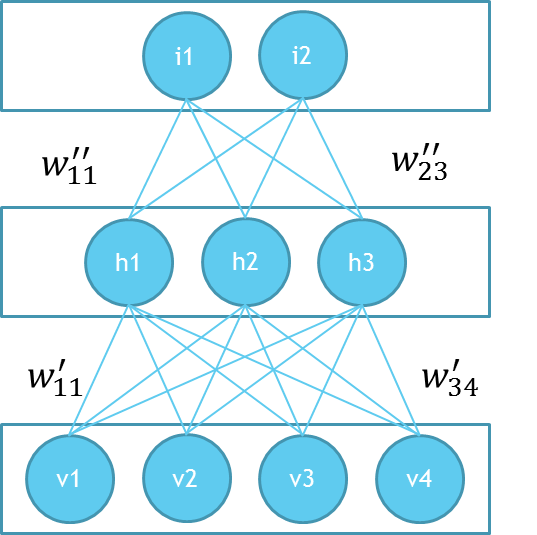
\includegraphics[width=0.95\textwidth]
		{pics/multistep2.png}
	\caption{Contoh Perhitungan tahap pertama dimulai dari top hidden unit }
	\label{fig:multistep2}
\end{figure}

\begin{figure}
	\centering
	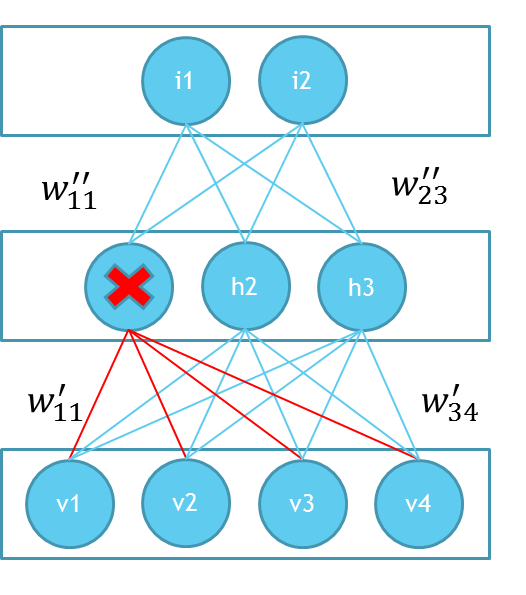
\includegraphics[width=0.95\textwidth]
		{pics/multistep3.png}
	\caption{Contoh Perhitungan tahap pertama dimulai dari top hidden unit }
	\label{fig:multistep3}
\end{figure}

Perhitungan diatas secara iteratif dilakukan mulai dari layer output mundur sampai layer input.

%-----------------------------------------------------------------------------%
\section{Implementasi Metode Perangkingan Bobot Secara Multi Step Untuk Mendapatkan Gen Biomarker}
%-----------------------------------------------------------------------------%
Implementasi multi-step ranking dengan menggunakan python:\\
Listing 3.4 : Implementasi Multi-Step Ranking di python
\lstinputlisting[language=python, frame=single, basicstyle=\tiny]{snip/multistep_rank.py}

Contoh implementasi multistep rank pada model yang disimpan pada file: \\
Listing 3.5: Implementasi Multistep rank Pada Model
\lstinputlisting[language=python, frame=single, basicstyle=\tiny]{snip/extractmodel.py}

%-----------------------------------------------------------------------------%
\section{Pengumpulan Data dan Pengolahan Awal}
%-----------------------------------------------------------------------------%
Data microarray tersedia secara bebas di \textit{GEO (Gene Expression Omnibus)} [http://www.ncbi.nlm.nih.gov/geo/], dan dapat diunduh, untuk digunakan sebagai data penelitian. Kemudian dilakukan normalisasi standar yang sering di pakai pada data \textit{microarray} dan yang sudah dibahas pada bab 2. Proses normalisasi ada banyak metode, dan akan digunakan satu metode standar untuk pengolahan awal microarray agar mendapatkan data konsisten dan dapat dibandingkan. Proses pengolahan awal dan normalisasi digunakan tools standar dan tersedia bebas yaitu R-Bioconductor. \\

\begin{figure}
	\centering
	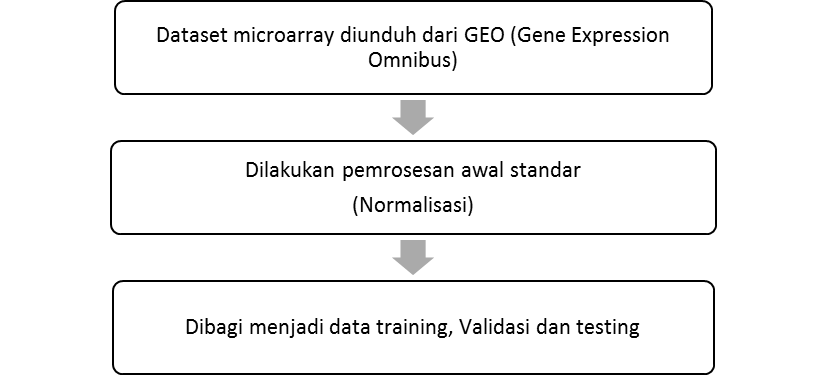
\includegraphics[width=0.9\textwidth]
		{pics/bagian1.png}
	\caption{Proses Pengumpulan data dan Pengolahan Awal}
	\label{fig:pengolahan_awal}
\end{figure}


%-----------------------------------------------------------------------------%
\section{Data Profil Gen Percobaan Microarray dan Biomarker}
%-----------------------------------------------------------------------------%

Definisi \textit{Biomarker} adalah sesuatu penanda yang bisa digunakan sebagai indikator suatu penyakit dari pasien. [http://www.biomarker.co.uk/whatisabiomarkers.html] Sebagai contoh, untuk mendiagnosa kanker paru-paru, hanya dibutuhkan 26 ekspresi gen saja. Gen yang paling informatif ini disebut dengan Biomarker (Bing, 2006). Pada profil gen GSE10072 yang merupakan kanker paru-paru, menurut  \citep{belinsky2004gene} ada 26 gen yang paling berpengaruh dari 22.283 gen yang diteliti secara bersamaan, seperti ditunjukkan pada \pic~\ref{fig:biomarker} yang merupakan contoh dari \textit{biomarker} kanker paru-paru.

\begin{figure}
	\centering
	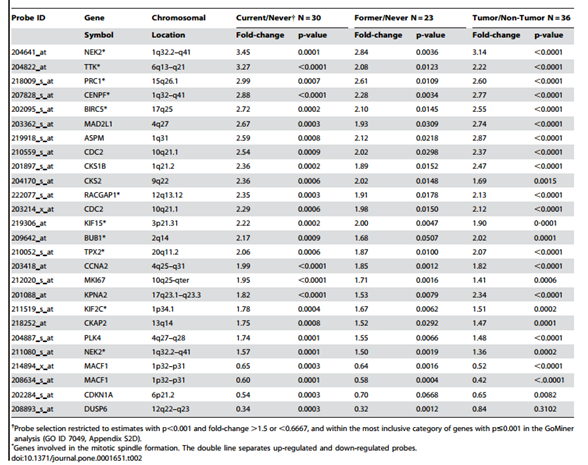
\includegraphics[width=1\textwidth]
		{pics/biomarker.png}
	\caption{Contoh 26 Gen Biomarker Kanker Paru-paru GSE10072 \citep{landi2008gene}}
	\label{fig:biomarker}
\end{figure}


%-----------------------------------------------------------------------------%
\section{Perancangan Metodologi Penelitian}
%-----------------------------------------------------------------------------%

%-----------------------------------------------------------------------------%
\subsection{Tahapan \textit{Unsupervised}}
%-----------------------------------------------------------------------------%
Tahap \textit{unsupervised} adalah tahapan dimana model DBN ditraining secara \textit{unsupervised} dengan data training pada tiap-tiap layernya secara \textit{greedy}, artinya, proses pelatihan dilakukan secara berjenjang mulai dari layer visibel dengan hidden layer 0 dan kemudian layer ini bobotnya dibuat tetap dan digunakan sebagai input pada leyer berikutnya. Tiap layernya dihitung \textit{cost}-nya, yang merupakan selisih dari error konstruksi dan error rekonstruksinya \citep{hinton2006fast} untuk kemudian diminimisasi errornya dengan menggunakan teknik \textit{Contrastive Divergence (CD)}. Konsep ini disebut \textit{greedy layer-wise training} yaitu setiap layer di traning secara independen dan satu-satu mulai dari layer input yang merupakan data ekspresi gen yang sudah disesuaikan dan dinormalisasi sampai layer output. Seperti pada \pic~\ref{fig:greedy1}

\begin{figure}
	\centering
	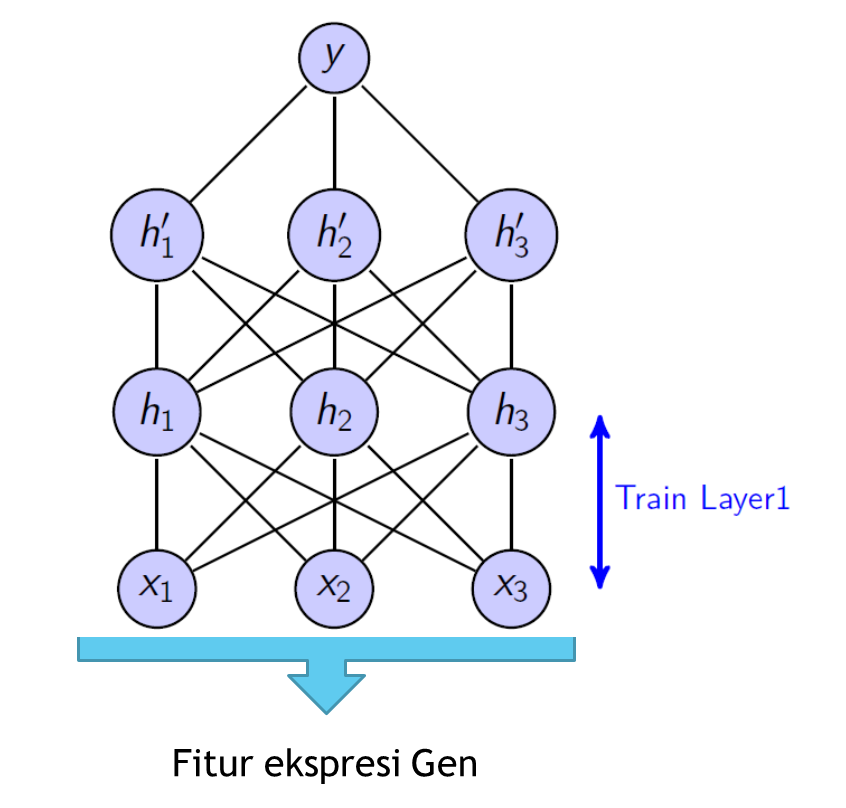
\includegraphics[width=0.5\textwidth]
		{pics/greedy1.png}
	\caption{Greedy layer-wise training pada layer visible dan hidden pertama\citep{duh2014deep}}
	\label{fig:greedy1}
\end{figure}

Setelah layer pertama selesai di training, layer pertama dibuat \textit{fixed} dan dipakai sebagai inputan visible dari layer selanjutnya. Demikian selanjutnya sampai layer terakhir yaitu layer output. Seperti pada \pic~\ref{fig:greedy2}

\begin{figure}
	\centering
	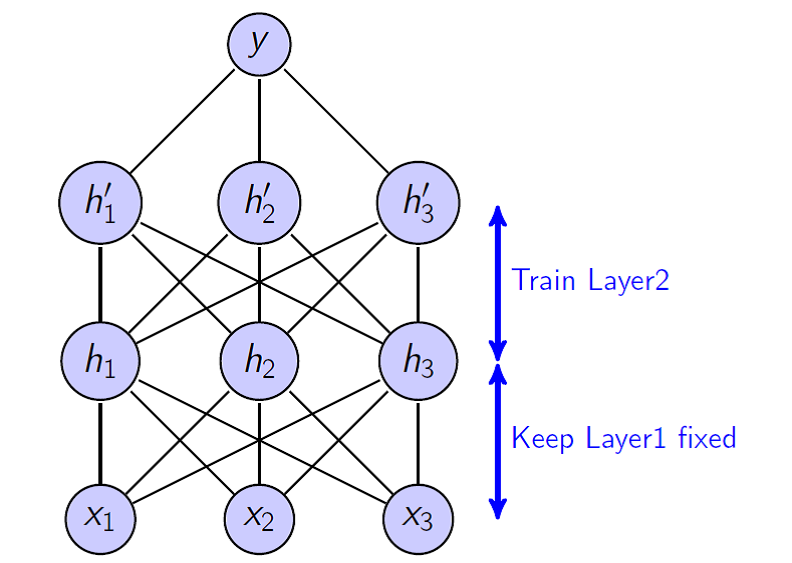
\includegraphics[width=0.5\textwidth]
		{pics/greedy2.png}
	\caption{Greedy layer-wise training pada selanjutnya, yaitu dengan membuat layer sebelumnya Fixed \citep{duh2014deep}}
	\label{fig:greedy2}
\end{figure}

Pada tahapan training secara unsupervised ini dihitung cost function antara error konstruksi dibandingkan dengan error rekonstruksinya. Dalam RBM yaitu error konstruksi atau disebut error fase positif dibandingkan dengan error rekonstruksi atau error fase negatif.\\ Fungsi cost yang digunakan pada percobaan ini adalah NLL. Dimana log-likelihood $\mathcal{L}(\theta, \mathcal{D})$ dan fungsi loss-nya sebagai NLL $\ell (\theta, \mathcal{D})$ sebagai berikut:

\begin{equation}
\begin{aligned}
\mathcal{L}(\theta, \mathcal{D}) &= \frac{1}{N} \sum_{x^{(i)} \in
\mathcal{D}} \log\ p(x^{(i)}) \\
\ell (\theta, \mathcal{D}) &= - \mathcal{L} (\theta, \mathcal{D})
\end{aligned}
\end{equation}


Menggunakan stochastic gradient $-\frac{\partial  \log p(x^{(i)})}{\partial
\theta}$, dimana $\theta$ adalah parameter dari modelnya.\\
Loss function yang merupakan Cost adalah  negative log-likelihood dari log-likelihood model. Data dari gradien NLL kemudian memiliki bentuk yaitu:
\begin{equation}
- \frac{\partial  \log p(x)}{\partial \theta}
 = \frac{\partial \mathcal{F}(x)}{\partial \theta} -
       \sum_{\tilde{x}} p(\tilde{x}) \
           \frac{\partial \mathcal{F}(\tilde{x})}{\partial \theta}.
\end{equation}

\subsubsection{Cost}
Cost merupakan variabel yang menggambarkan \textit{Negative Log Likelihood}. Yang memiliki bentuk persamaan sebagai berikut:
\begin{equation}
\frac{1}{|\mathcal{D}|} \mathcal{L} (\theta=\{W,b\}, \mathcal{D}) =
            \frac{1}{|\mathcal{D}|} \sum_{i=0}^{|\mathcal{D}|}
                \log(P(Y=y^{(i)}|x^{(i)}, W,b)) \\
            \ell (\theta=\{W,b\}, \mathcal{D})
\end{equation}

Dalam kode python dituliskan:
\begin{center}
cost = classifier.negative\_log\_likelihood(y)
\end{center}

Semakin kecil cost, menunjukkan semakin kecil error rekonstruksinya. Hal ini menunjukkan bahwa, data rekonstruksi mendekati bentuk data konstruksinya (diambil dari data training).


%-----------------------------------------------------------------------------%
\subsection{Tahapan Supervised}
%-----------------------------------------------------------------------------%
Pada saat \textit{training}  secara \textit{unsupervised} dilakukan, diukur \textit{cost} yang menunjukkan perbedaan antara konstruksi dan rekonstruksi pada tiap layernyanya. Akan tetapi, hal ini hanya untuk mengetahui \textit{cost} tiap-tiap layer RBM-nya, bukan seberapa baik model dalam melakukan klasifikasi. Oleh karena itu diperlukan satu layer output yang yang berupa \textit{logistic regression} untuk mengetahui seberapa baik model dalam membedakan pasien kelas kanker dan normal.

\subsubsection{Implementasi Logistic Regression pada Layer Output}

Logistic regression adalah klasifier linear yang memiliki matriks bobot $W$ dan vektor bias $b$. Klasifikasi merupakan proyeksi titik data pada sebuah himpunan \textit{hyperplane} yang jaraknya digunakan sebagai penentu probabilitas keanggotaan kelasnya. Secara matematis bisa dituliskan sebagai:
\begin{equation}
\begin{aligned}
  P(Y=i|x, W,b) &= softmax_i(W x + b) \\
                &= \frac {e^{W_i x + b_i}} {\sum_j e^{W_j x + b_j}}
\end{aligned}
\end{equation}

Output dari model akan memprediskikan dengan menghitung \textit{argmax} dari vektor dimana elemen ke $i$ adalah $P(Y=i|x)$.
\begin{equation}
  y_{pred} = argmax_i  P(Y=i|x,W,b)
\end{equation}

Implementasinya menggunakan optimisasi stochastic gradient descent. Untuk implementasi lengkapnya ada di lampiran.

%-----------------------------------------------------------------------------%
\subsection{Tahapan Tuning Parameter}
%-----------------------------------------------------------------------------%
Parameter yang akan dilakukan \textit{tuning} disini adalah: jumlah hidden units, jumlah banyaknya layer hidden dan banyaknya epoch. Tuning parameter dilakukan agar bisa didapatkan hasil yang optimum dari percobaan yang dilakukan. Tahap ini adalah tahap yang paling krusial untuk mendapatkan hasil yang diinginkan. Dikarenakan uniknya data microarray, maka  dilakukan \textit{trial and error} dari parameter-parameternya.\\
Proses tuning parameter ini memerlukan waktu yang lama karena setiap percobaan memiliki parameter yang diubah-ubah untuk menyesuaikan hasil yang diinginkan. Dikarenakan sifat dari microarray yang berbeda dengan citra yang sudah banyak dilakukan oleh peneliti, tuning parameter untuk data \textit{microarray} pada arsitektur deep learning jarang dilakukan oleh peneliti, sehingga proses tuning dilakukan setiap selesai dilakukan percobaan yang memerlukan waktu antara 2 hari sampai 5 hari, tergantung dari epoch dan jumlah layer dan hidden unitnya.\\
Proses training pada arsitektur \textit{deep learning} juga memerlukan kekuatan komputasi komputer yang kuat dan memory yang relatif lebih besar untuk mendapatkan model yang optimal. 



%-----------------------------------------------------------------------------%
\section{Melakukan Testing Arsitektur DBN}
%-----------------------------------------------------------------------------%
Hasil dari unsupervised learning yang dilakukan oleh DBN, akan diuji dahulu dengan dengan data validasi, apakah error rekonstruksinya lebih baik seperti pada gambar \ref{fig:overview}. Setelah dilakukan perankingan \textit{biomarker}, diperlukan pengujian apakah apakah seleksi fitur tersebut menggambarkan hasil yang diinginkan, dengan membandingkan biomarker yang dihasilkan dengan literature. 



%-----------------------------------------------------------------------------%
\section{Evaluasi Hasil Perangkingan Dengan Klasifikasi Secara Supervised Menggunakan MLP}
%-----------------------------------------------------------------------------%

Proses evaluasi dilakukan dua kali, pertama, saat menggunakan data asli tanpa seleksi fitur, yang kedua setelah dilakukan seleksi fitur. Hal ini dilakukan untuk mengetahui apakah seleksi fitur tersebut bisa memperbaiki hasil klasifikasi secara signifikan dibandingkan tanpa dilakukan seleksi fitur. \\
Evaluasi hasil hasil perankingan secara \textit{supervised} diperlukan untuk mengetahui apakah hasil perankingan tersebut memperbaiki hasil klasifikasi pasien kanker dan sehat hanya dengan menggunakan gen-gen yang dipilih berdasarkan ranking yang didapatkan.


%-----------------------------------------------------------------------------%
\section{Perbandingan Hasil Perangkingan Dengan Literatur}
%-----------------------------------------------------------------------------%
\begin{figure}
	\centering
	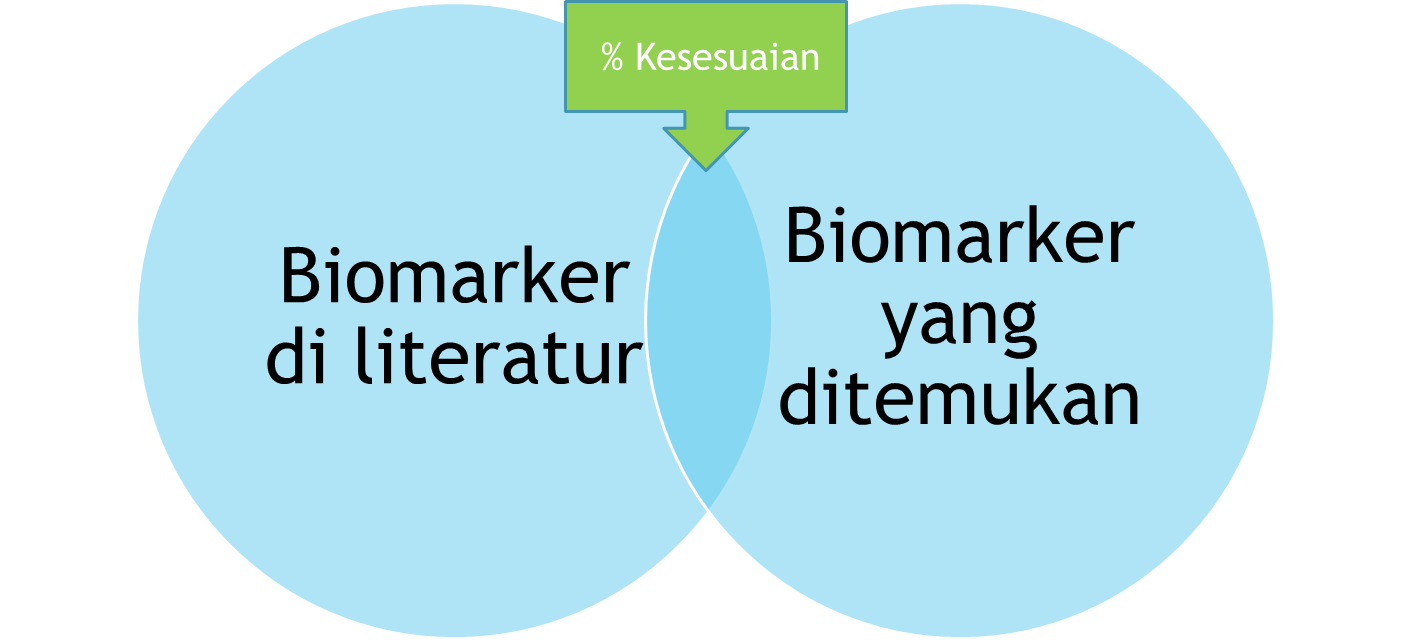
\includegraphics[width=0.9\textwidth]
		{pics/biomarker1.png}
	\caption{Persen Kesesuaian Antara Biomarker yang Ditemukan dibandingkan dengan Biomarker di Literatur}
	\label{fig:biomarker1}
\end{figure}

Hasil perankingan pada percobaan tersebut selanjutnya diteliti apakah gen hasil perankingan tersebut adalah gen yang memiliki signifikansi terhadap penyakit yang diinginkan. Dalam kasus ini yaitu penyakit kanker paru-paru. Berikut adalah contoh 26 gen biomarker pada percobaan GSE10072 yang disitasi dari paper \citep{landi2008gene}. 

%-----------------------------------------------------------------------------%
\section{Modul-modul Pendukung}
%-----------------------------------------------------------------------------%
\subsection{Kelas Ekstraktor}
Untuk melakukan pengolahan pengolahan awal, didevelop sebuat kelas yang bernama kelas Ekstraktor. Kelas ini berfungsi untuk mengekstrak file csv dari data gen, menjadi file yang memiliki struktur data yang sesuai dengan library dbn.py di python. Hal ini dilakukan agar datanya memiliki struktur yang sesuai dengan dbn yaitu dilakukan normalisasi data profil gen yang berbentuk ekspresi gen menjadi rentang antara 0 sampai 1.

\begin{figure}
	\centering
	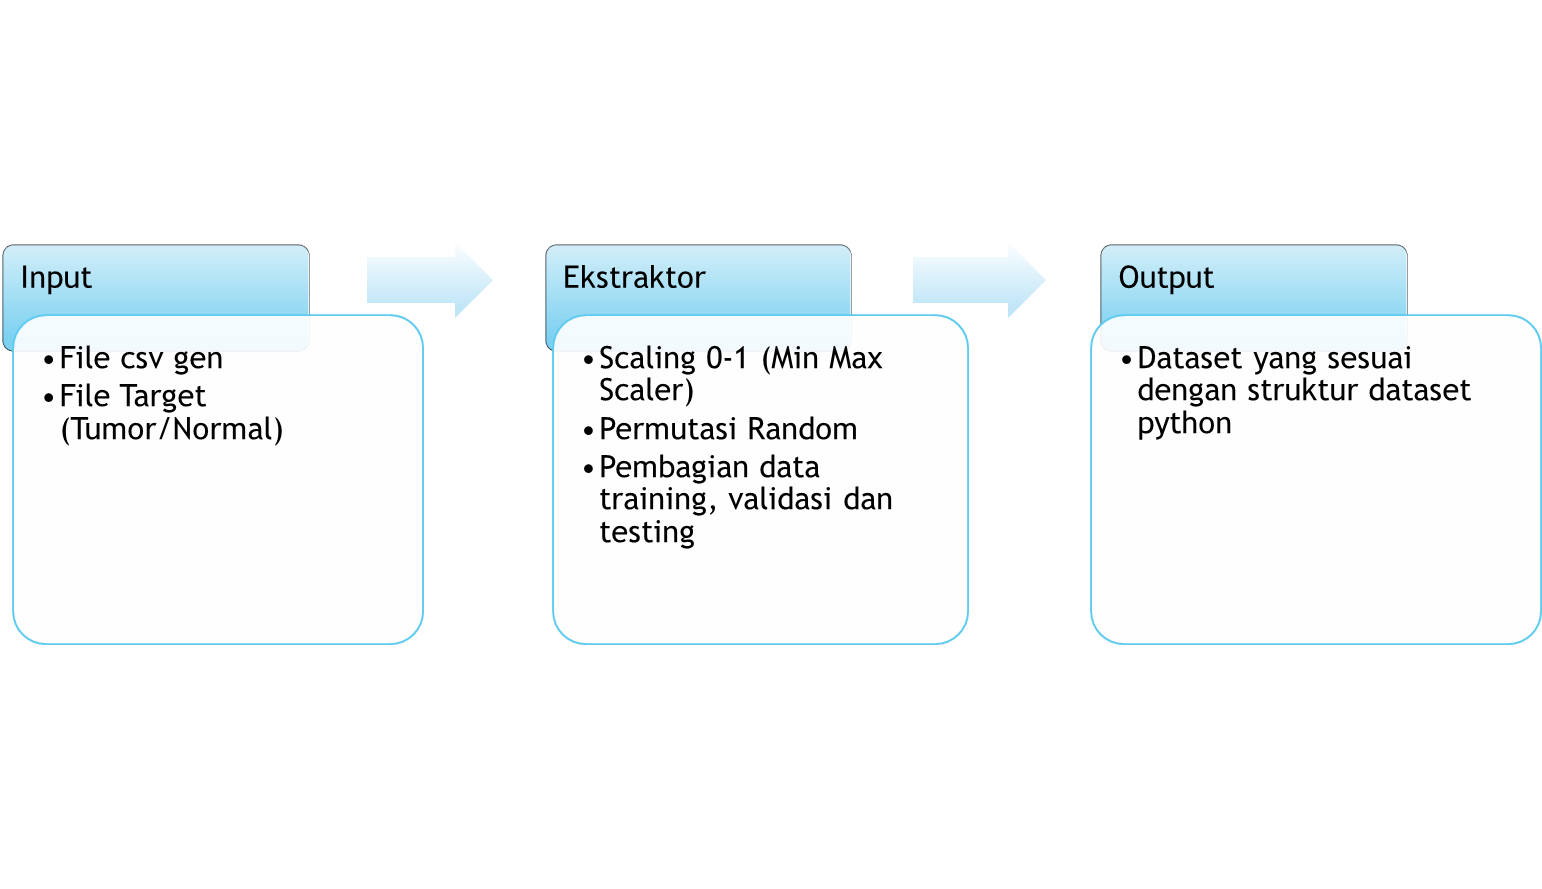
\includegraphics[width=0.9\textwidth]
		{pics/ekstraktor.png}
	\caption{Kelas Ekstraktor, Untuk melakukan Ekstraksi data Gen}
	\label{fig:preproses}
\end{figure}

\subsection{Implementasi Kelas Ekstraktor di Python}
Listing 4.1: Ekstraksi dataset untuk disesuaikan dengan struktur data modul dbn.py
\lstinputlisting[language=python, frame=single, basicstyle=\tiny]{snip/ekstrak_csv.py}

Kelas ekstraktor ini melakukan adaptasi data yang tadinya memiliki struktur yang tidak kompatibel dengan library Theano yang di python, menjadi kompatibel dan memiliki struktur data yang disesuaikan. Kemudian, dilakukan juga permutasi random agar datanya memiliki sebaran yang normal untuk kemudian dilakukan pembagian data yang terdiri dari sekian persen data training, validasi dan testing.

\subsection{Kelas Generator}
Kelas Generator ini adalah modul yang dibuat agar bisa secara otomatis memilih gen-gen yang dianggap penting pada sebuah array yang berisi index dari gen yang ada pada dataset.
\begin{figure}
	\centering
	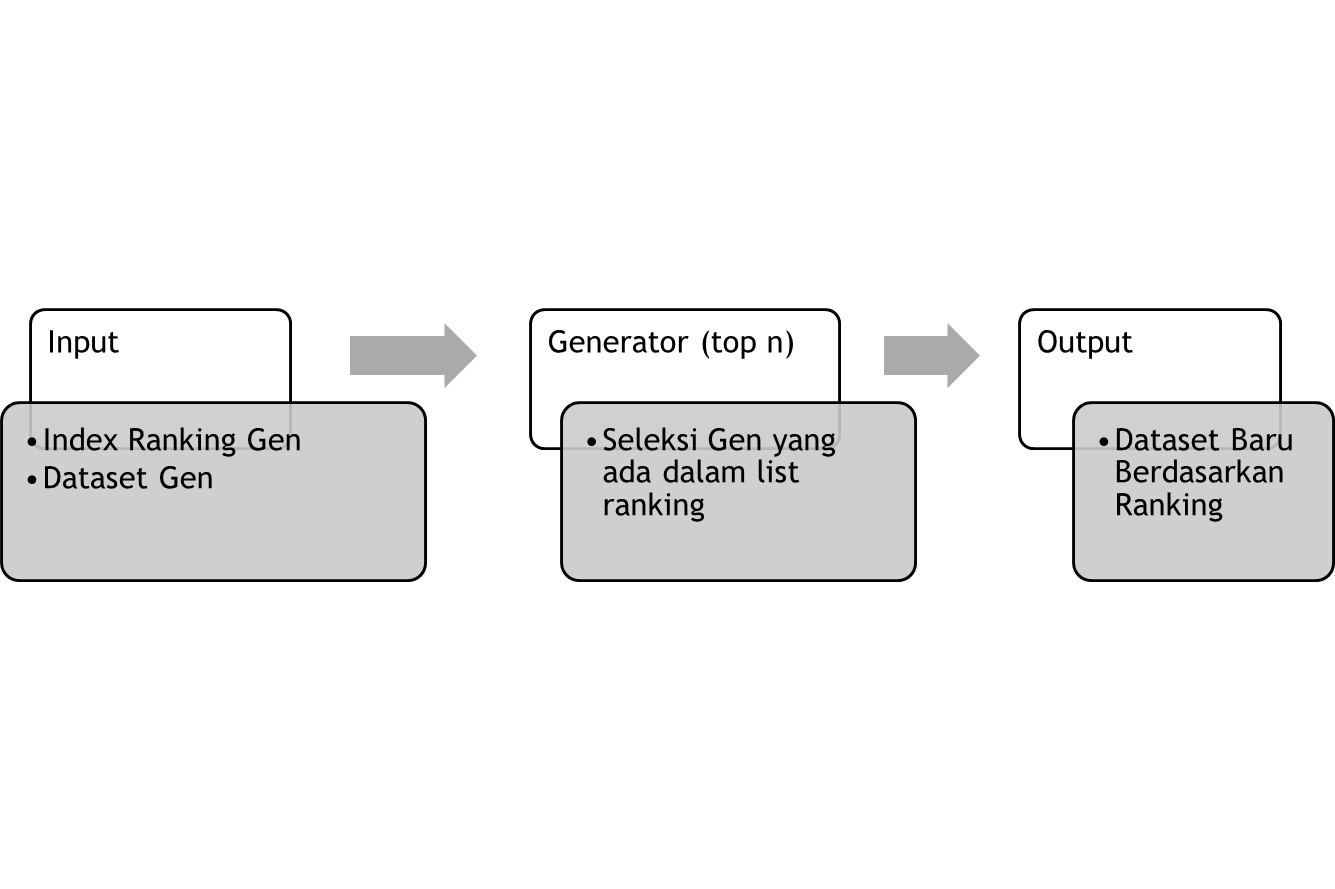
\includegraphics[width=0.8\textwidth]
		{pics/generator.png}
	\caption{Diagram Kelas Generator yang digunakan untuk menggenerasi data gen berdasarkan rankingnya}
	\label{fig:generator}
\end{figure}


\subsection{Hasil Evaluasi Dengan Multi Layer Perceptron}

\begin{figure}
	\centering
	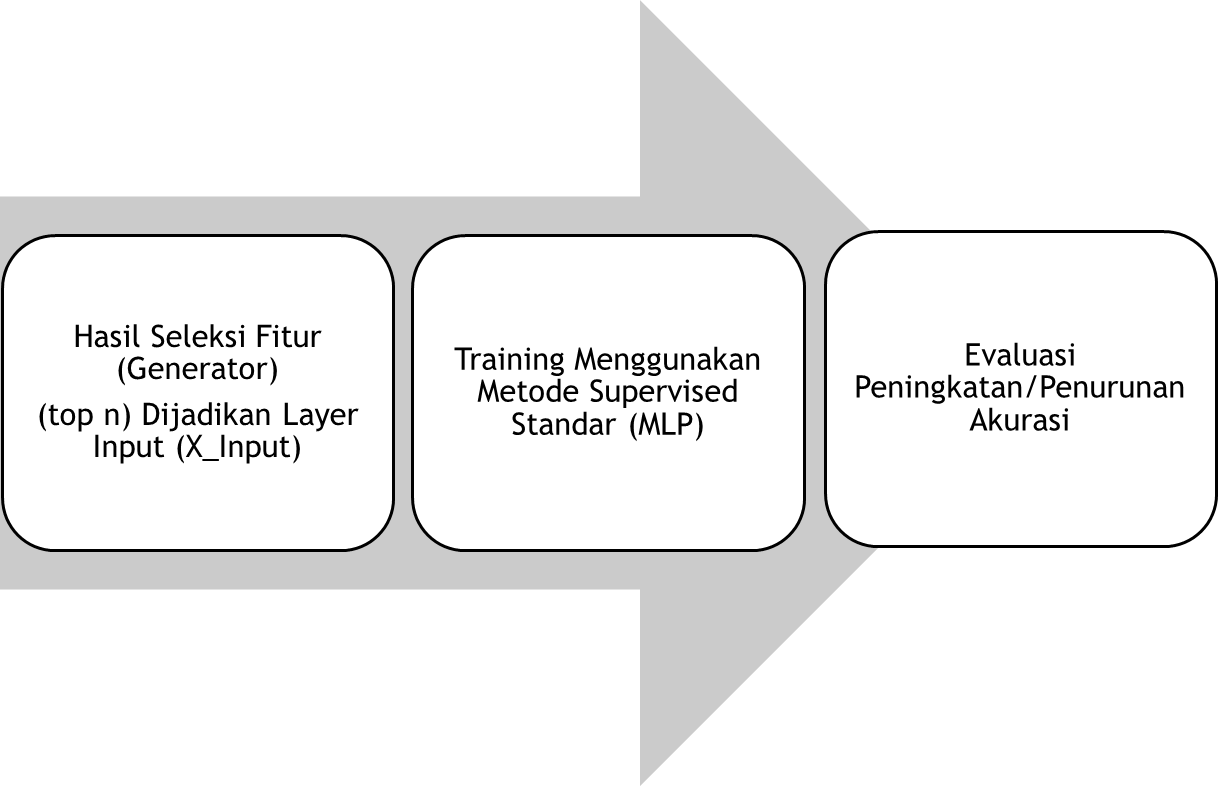
\includegraphics[width=0.7\textwidth]
		{pics/generator2.png}
	\caption{Diagram Proses Menggenerasi Data Untuk Dijadikan Dataset Training}
	\label{fig:generator2}
\end{figure}
Setelah didapatkan top-n gen, diperlukan proses untuk menggenerasi data ulang yang didapat dari data asli diambil gen top-n tersebut, pada penelitian ini akan diambil top 250 gen agar sesuai dengan gen yang didapat di literatur untuk kemudian dilakukan konfirmasi. Dan dievaluasi apakah terjadi peningkatan atau penurunan akurasi dibandingkan dengan tanpa adanya seleksi fitur.






